\section{Tobii Eye Tracker 5} \label{sec:hwds_TobiiEyeTracker5}

\begin{figure}[h]
    \centering
    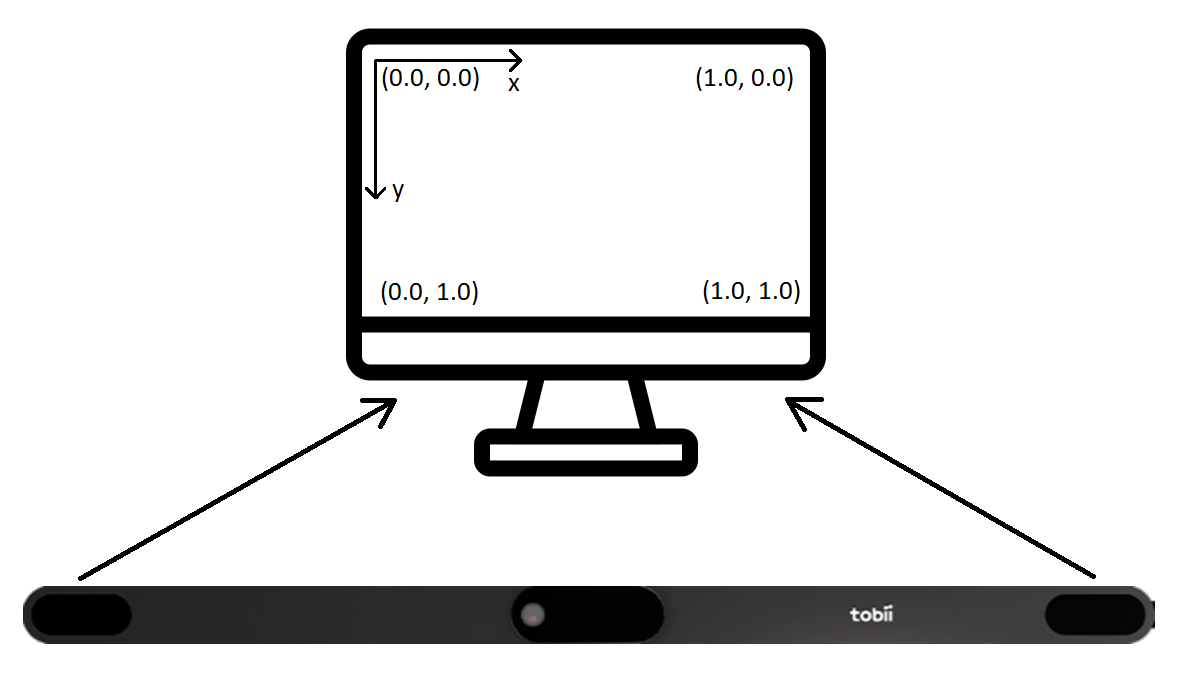
\includegraphics[width=0.8\textwidth]{Images/hwds_hardware.png}
    \caption{Hardware of Tobii Eye Tracker 5, as well as a depiction of its setup.}
    \label{fig:hwds_hardware}
\end{figure}

The eye-tracking hardware used for the entirety of this thesis is the \textit{Tobii Eye Tracker 5} (Tobii ET5), shown in figure \ref{fig:hwds_hardware}. It is produced by a Swedish company with 20 years of experience, which is currently the only actor in the market to make low-cost eye-trackers. They have had this position since mid-2014. Released in July 2020, Tobii ET5 is their third iteration in low-cost commercial-grade eye-tracking hardware.

Tobii ET5 features two 850nm near-infrared light illuminators in a stereo configuration, roughly 25cm apart. Between these illuminators is an optical biometric face sensor. Together they allow for remote eye tracking without any intrusions on the subject, allowing for free movement within a given head-box. Remote eye-tracking is possible due to the pupil- and corneal reflection method of gaze estimation, supported by head pose estimation by a convolutional neural network. The head-box is defined as roughly 60-80cm from the monitor and about 30cm vertically and laterally. From there, the tracker can estimate gaze in a 35x35cm on-screen track-box. That is enough to cover monitor sizes up to a maximum of 27", with an aspect ratio of 16:9. It records head position at 133Hz. However, gaze estimation is still limited to 33Hz due to a limitation in the illuminator emission frequencies. It is mounted directly below the monitor, as shown in figure \ref{fig:hwds_hardware}.

\subsection{Data Output}

Data from Tobii ET5 is output at 33Hz, in on-screen coordinates by the coordinate system shown in figure \ref{fig:hwds_hardware}. Upon installation, between subjects and otherwise as often as possible, a calibration is required to get accurate gaze estimations. There is an average interval of about 30ms between samples in regular operation. Samples are excluded from the data stream for data points where the tracker does not detect a pupil or gaze beyond the track-box to which it is calibrated. Once the pupil is again visible, or the subject returns their gaze within the track-box, the tracker requires some time to recover a gaze estimation. As such, intervals of missing data samples are not necessarily suitable measures of actual blink duration.

Additionally, data is lightly filtered to remove noise. Sadly, the details of this processing are not publicly available to the customer for Tobii's low-cost eye trackers. 